\documentclass[a4paper,11pt]{article}
\usepackage[utf8]{inputenc}
\usepackage[left=2cm,text={17cm, 24cm},top=3cm]{geometry}

\usepackage{float}
\usepackage{caption}
\usepackage{graphicx}
\usepackage{amsmath}
\usepackage{amsfonts}
\usepackage{amsthm}
\usepackage{multirow}
\usepackage{times}
\usepackage{verbatim}
\usepackage[czech]{babel}
\usepackage[ruled,vlined,linesnumbered,czech,longend]{algorithm2e}

\usepackage{pdflscape}

\newcommand{\myuv}[1]{\quotedblbase #1\textquotedblleft}

\author{Martin Bažík \\ xbazik00@stud.fit.vutbr.cz}
\title{Typografie a publikování \\ 2. projekt}
\date{}


\begin{document}
	\begin{titlepage}
		\begin{center}
			\textsc{\Huge Vysoké učení technické v~Brně}\\
			\textsc{\huge Fakulta informačních technologií}
					\vspace{\stretch{0.382}}
			\\{\LARGE Typografie a publikování -- 3. projekt\\
				\Huge Tabulky a obrazky }
			\vspace{\stretch{0.618}}
		\end{center}
		{\Large 2. dubna 2016 \hfill Martin Bažík}	
	\end{titlepage}
	\newpage	
	
	\section{Úvodní strana}
	Název práce umístěte do zlatého řezu a nezapomeňte uvést dnešní datum a vaše jméno a příjmení.
	
	\section{Tabulky}
	Pro sázení tabulek můžeme použít buď prostředí \texttt{tabbing} nebo prostředí \texttt{tabular}.
	
	\subsection{Prostředí \texttt{tabbing}}
	Při použití \texttt{tabular} vypadá tabulka následovně:
	
	\begin{tabbing}
		\textbf{Ovoce} \qquad\qquad \= \textbf{Cena} \quad \= \textbf{Množství} \\
		Jablka \> 25,90 \> 3 kg \\
		Hrušky \> 27,40 \> 2,5 kg \\
		Vodní melouny \> 35,-- \> 1 kus  
	\end{tabbing}
	
	Toto prostředí se dá také použít pro sáyení algoritmů, ovšem vhodnejší je použít prostředí \texttt{algorithm}
	nebo \texttt{algorithm2e} (viz sekce \ref{sek:3}).
	
	\subsection{Prostředí \texttt{tabular}}
	
	Další možností, jak vztvořit tabulku, je použít prostředí \texttt{tabular}. Tabulky pak budou vypadat takto\footnotemark. 
	
	\begin{table}[ht]
		\catcode`\-=12
		\begin{center}
			\begin{tabular}{| l | r | r |}
				\hline
				 & \multicolumn{2}{|c|}{\textbf{Cena}} \\\cline{2-3} 
				\textbf{Měna} & \textbf{nákup} & \textbf{prodej} \\ \hline
				EUR & 27,34 & 27,42 \\
				GBP & 33,09 & 33,21 \\
				USD & 19,87 & 19,95 \\\hline
			\end{tabular}
			\caption{Tabulka kurzů k~dnešnímu dni}
			\label{tabKurzu}
		\end{center}
	\end{table}
	
	\begin{table}[ht]
		\catcode`\-=12
		\begin{center}
			\begin{tabular}{| c | c |}
				\hline
				$A$ & $\neg A$ \\
				\hline
				\textbf{P} & N \\
				\hline
				\textbf{O} & O~\\
				\hline
				\textbf{X} & X \\
				\hline
				\textbf{N} & P \\
				\hline
				
			\end{tabular}
			\begin{tabular}{| c | c | c | c | c | c |}
				\hline
				\multicolumn{2}{|c|}{\multirow{2}{*}{$A \wedge B$}}& \multicolumn{4}{|c|}{$B$}\\
				\cline{3-6}
				\multicolumn{2}{|c|}{} & \textbf{P} & \textbf{O} & \textbf{X} & \textbf{N}\\
				\hline
				\multirow{4}{*}{$A$} & \textbf{P} & P & O~& X & N \\
				\cline{2-6}
				& \textbf{O} & O~& O~& N & N \\
				\cline{2-6}
				& \textbf{X} & X & N & X & N \\
				\cline{2-6}
				& \textbf{N} & N & N & N & N \\
				\hline
			\end{tabular}
			\begin{tabular}{| c | c | c | c | c | c |}
				\hline
				\multicolumn{2}{|c|}{\multirow{2}{*}{$A \vee B$}}& \multicolumn{4}{|c|}{$B$}\\
				\cline{3-6}
				\multicolumn{2}{|c|}{} & \textbf{P} & \textbf{O} & \textbf{X} & \textbf{N}\\
				\hline
				\multirow{4}{*}{$A$} & \textbf{P} & P & P & P & P \\
				\cline{2-6}
				& \textbf{O} & P & O~& P & O~\\
				\cline{2-6}
				& \textbf{X} & P & P & X & X \\
				\cline{2-6}
				& \textbf{N} & P & O~& X & N \\
				\hline
			\end{tabular}
			\begin{tabular}{| c | c | c | c | c | c |}
				\hline
				\multicolumn{2}{|c|}{\multirow{2}{*}{$A \to B$}}& \multicolumn{4}{|c|}{$B$}\\
				\cline{3-6}
				\multicolumn{2}{|c|}{} & \textbf{P} & \textbf{O} & \textbf{X} & \textbf{N}\\
				\hline
				\multirow{4}{*}{$A$} & \textbf{P} & P & O~& X & N \\
				\cline{2-6}
				& \textbf{O} & P & O~& P & O~\\
				\cline{2-6}
				& \textbf{X} & P & P & X & X \\
				\cline{2-6}
				& \textbf{N} & P & P & P & P \\
				\hline
			\end{tabular}
			\caption{Protože Kleeneho trojhodnotová logika už je \myuv{zastaralá}, uvádíme si zde příklad čtyřhodnotové logiky}
			\label{tabPrav}
		\end{center}
	\end{table}
	\footnotetext{Kdyby byl s~\texttt{cline}, zkuste se podívat třeba sem: http://www.abclinuxu.cz/tex/poradna/show/325037.}
	
	\section{Algoritmy}\label{sek:3}
	
	Pokud budeme chtít vysázet algoritmus, můžeme použít prostředí \texttt{algorithm\footnotemark} nebo \texttt{algorithm2e\footnotemark}.
	Příklad použití prostředí \texttt{algorithm2e} viz Algoritmus \ref{algo:max}.
	\footnotetext{
		Pro nápovědu, jak zacházet s~prostředím algorithm, můžeme zkusit tuhle stránku:\\
		http://ftp.cstug.cz/pub/tex/CTAN/macros/latex/contrib/algorithms/algorithms.pdf.
	}
	\footnotetext{
		Pro algorithm2e zase tuhle: http://ftp.cstug.cz/pub/tex/CTAN/macros/latex/contrib/algorithm2e/doc/algorithm2e.pdf.
	}
	
	
	\SetNlSty{text}{}{:}
	\SetAlgoNoLine
	\SetNlSkip{-1em}

	\begin{algorithm}
		\DontPrintSemicolon % Some LaTeX compilers require you to use \dontprintsemicolon instead
		
		\KwIn{$(X_{t-1},u_t,z_t)$}
		\KwOut{$X_t$}
		\Indentp{1.5em}
		$\overline{X_t}=X_t=0$\;
		\For{$k=0\; \mathrm{to}\; M$} {
			$x^{\left[k\right]}=sample_motion_model(u_t,x_{t-1}^{\left[k\right]})$ \;
			$w^{\left[k\right]}=measurement_model(z_t,x_t^{\left[k\right]},m_{t-1})$ \;
			$m^{\left[k\right]}=updated_occupancy_grid(z_t,x_t^{\left[k\right]},m_{t-1}^{\left[k\right]})$ \;
			$\overline{X_t}=\overline{X_t}+\langle x_{x}^{\left[m\right]},w_{t}^{\left[m\right]}\rangle$
		}
		\For{$k=0\; \mathrm{to}\; M$} {
		draw $i$ with probability $\approx w_{t}^{\left[i\right]}$ \;
		add $\langle x_{x}^{\left[k\right]},m_{t}^{\left[k\right]}\rangle$ to $X_t$ 
		}
		\Return $X_t$
		\caption{{\sc Fast}SLAM}
		\label{algo:max}
	\end{algorithm}
	
	\section{Obrázky}
	Do našich článků můžete samozřejme	vkládat obrázky. Pokud je obrázkem fotografie, můžete klidně použít bitmapový soubor. Pokud by to ale mělo být nějaké schéma nebo něco podobného, je dobrým zvykem takovýto obrázek vytvořit vektorově.
	\begin{figure}[H]
		
		\centering
		\scalebox{0.4}{
		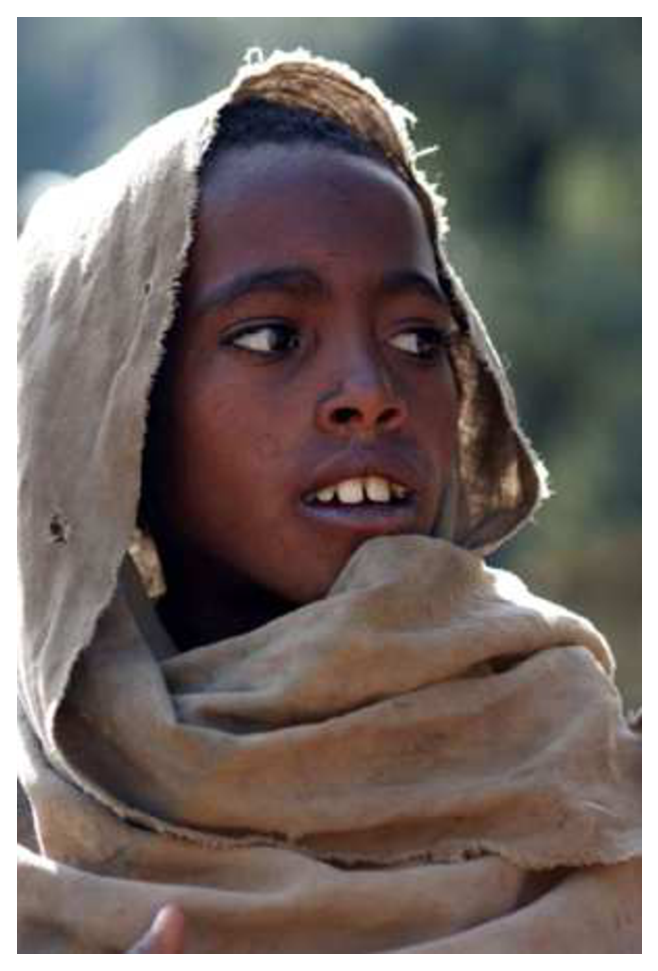
\includegraphics{etiopan}
		\reflectbox{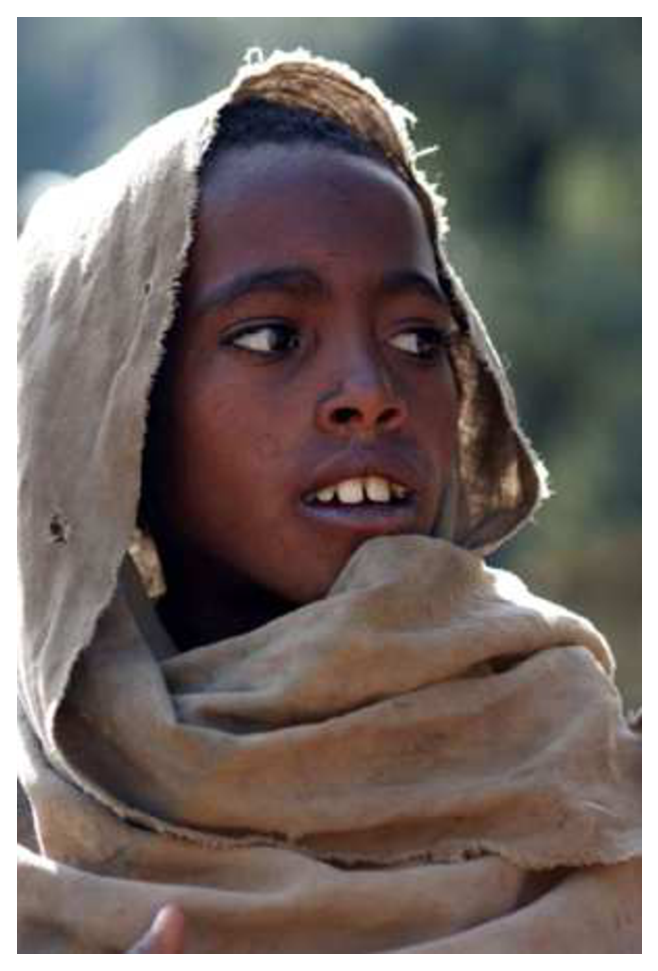
\includegraphics{etiopan}}}
		\caption{Malý Etiopánek a jeho bratříček}
		\label{picEtiopan}
	\end{figure}
	\newpage
	\noindent
	Rozdíl mezi vektorovým ...
	\begin{figure}[H]
		\centering
		
\includegraphics[scale=0.4]{oniisan}	
		\caption{Vektorový obrázek}
		\label{picVector}
	\end{figure}
	\noindent
	... a bitmapovým obrázkem
	\begin{figure}[H]
		\centering
		
\includegraphics[scale=0.6]{oniisan2}	
		\caption{Bitmapový obrázek}
		\label{picBitmap}
	\end{figure}
	\noindent
	se projeví při zvětšení.
	
	Odkazy (nejen ty) na obrázky \ref{picEtiopan}, \ref{picVector} a \ref{picBitmap}, na tabulky \ref{tabKurzu} a \ref{tabPrav} a také algoritmus \ref{algo:max} jsou udělány pomocí křížových odkazů. Pak je ovšem potřeba zdrojový soubor přeložit dvakrát.
	
	Vektrové obrázky lze vytvořit i přímo v~\LaTeX u, například pomocí prostředí \texttt{picture}.
	\newpage
	\begin{landscape}
		\begin{figure}[H]
			\centering
			\setlength{\unitlength}{5cm}
			\begin{picture}(4,2.3)
				\framebox(4,2){
				\linethickness{1.5mm}
				\put(-1.9,-1.4){\line(1,0){3.8}}
				\linethickness{0.6mm}
				\put(-1.5,-1.4){\line(0,1){0.6}}
				\put(-1.5,-0.8){\line(1,0){0.8}}
				\put(-0.7,-0.89){\framebox(1,0.2){}}
				\put(0.31,-0.89){\framebox(1,0.05){}}
				\put(-1.1,-1.0){\framebox(2.8,0.1){}}
				\put(-1.11,-1.01){\line(1,-1){0.2}}
				\put(-1.2,-1.4){\line(0,1){0.2}}
				\put(-1.2,-1.2){\line(1,0){0.5}}
				\put(-0.7,-1.2){\line(3,-1){0.6}}
				\put(-0.65,-1.2166){\line(0,1){0.1766}}
				\put(-0.65,-1.04){\line(1,0){2.3}}
				\put(1.65,-1.04){\line(0,-1){0.25}}
				\put(1.7,-1.4){\line(0,1){0.11}}
				\put(1.7,-1.29){\line(-1,0){2.1266}}
				\put(1.5,-0.1){\circle{0.5}}
				}
			\end{picture}
			\caption{Vektorový obrázek v~prostředí \texttt{picture}}
			\label{picVec2}
		\end{figure}
	\end{landscape}
\end{document}
%ů